\begin{frame}{Selection dileptau}
  \begin{columns}
    \begin{column}{0.5\textwidth}
      \centering 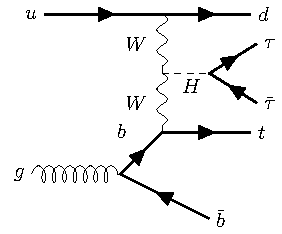
\includegraphics[width=0.9\textwidth]{/cephfs/user/s6chkirf/feynman_diagrams/tHq_tautau}\\
      \begin{itemize}
        \item n-jets: 2-6 (b-jets: \textbf{1})
        \item b-jet WP: 70 DL1r
        \item nLeptons \& nTaus: $\bf{2e / \mu~1\tau_{\text{had}}} $(1 OS light lepton)
        \item $E_{\text{T,miss}}$: no cut (to \SI{800}{GeV})
      \end{itemize}
    \end{column}
    \begin{column}{0.7\textwidth}
      \vspace*{-0.05\textwidth}
      \begin{itemize}
        \footnotesize
        \item jets:
        \vspace*{-0.02\textwidth}
        \begin{itemize}
          \footnotesize
          \item $p_T>\SI{25}{GeV}$
          \item $|\eta|<4.5$
          \item EMPFlow
        \end{itemize}
        \item electrons:
        \vspace*{-0.02\textwidth}
        \begin{itemize}
          \footnotesize
          \item $p_T>\SI{20}{GeV}$ trigger matched \SI{27}{GeV}
          \item $|\eta|<2.5$ not in 1.37 - 1.52
          \item WP: Tight ; \\isolation: PLIVTight
        \end{itemize}
        \item muons:
        \vspace*{-0.02\textwidth}
        \begin{itemize}
          \footnotesize
          \item $p_T>\SI{20}{GeV}$ trigger matched \SI{27}{GeV}
          \item $|\eta|<2.5$
          \item WP: Tight ; isolation: PLIVTight
        \end{itemize}
        \item taus:
        \vspace*{-0.02\textwidth}
        \begin{itemize}
          \footnotesize
          \item $p_T>\SI{20}{GeV}$ trigger matched \SI{27}{GeV}
          \item $|\eta|<2.5$ not in 1.37 - 1.52
          \item WP: RNNMedium
          \item ASG recommended OLR ($\tau_{had}$ remove jets)
        \end{itemize}
      \end{itemize}
    \end{column}
  \end{columns}
\end{frame}
\begin{frame}{Features}
    \begin{columns}
        \begin{column}{0.5\textwidth}
            \resizebox{\linewidth}{!}{
            \begin{tabular}{|l|l|}
                \hline
                eta\_jf               & forward jet eta                        \\ \hline
                pt\_jf                & forward jet transverse momentum        \\ \hline
                mass\_jf              & forward jet mass                       \\ \hline
                phi\_jf               & forward jet phi                        \\ \hline
                eta\_b                & b-jet eta                              \\ \hline
                pt\_b                 & b-jet transverse momentum              \\ \hline
                mass\_b               & b-jet mass                             \\ \hline
                phi\_b                & b-jet phi                              \\ \hline
                MMC\_out\_1             & reconstructed Higgs mass               \\ \hline
                m\_met                & Missing energy                         \\ \hline
                met\_x                & Missing energy x-component             \\ \hline
                met\_y                & Missing energy y-component             \\ \hline
                Reco\_w\_Tmass\_1     & Reconstructed Tmass of the W case 1    \\ \hline
                Reco\_w\_mass\_1      & Reconstructed mass of the W case 1     \\ \hline
            \end{tabular}}
        \end{column}
        \begin{column}{0.5\textwidth}
            \resizebox{\linewidth}{!}{
            \begin{tabular}{|l|l|}
                 \hline
                 deltaRTau            & Delta R of the hadronic taus          \\ \hline
                 deltaPhiTau          & Delta phi of the hadronic taus        \\ \hline
                 HvisPt               & pt of LorentzV sum of hadronic taus   \\ \hline
                 HvisEta              & eta of LorentzV sum of hadronic taus  \\ \hline
                 TvisMass             & mass of reconstructed top             \\ \hline
                 TvisPt               & pt of visible top                     \\ \hline
                 TvisEta              & eta of visible top                    \\ \hline
                 fs\_had\_tau\_1\_pt  & Hadronic tau pt                       \\ \hline
                 fs\_had\_tau\_1\_eta & Hadronic tau eta                      \\ \hline
                 fs\_had\_tau\_1\_m   & Hadronic tau m                        \\ \hline
                 lep\_Top\_pt         & Light lepton pt                       \\ \hline
                 lep\_Top\_eta        & Light lepton eta                      \\ \hline
             \end{tabular}}
        \end{column}
    \end{columns}
    \begin{itemize}
      \item Experimented with many setups.
      \item Ranking is planned for documentation but no improvement is expected
    \end{itemize}
\end{frame}


\begin{frame}{Lephad Hyperparameters}
    \begin{table}[]
    \begin{tabular}{|l|l|}
    \hline
    Hyperparameter          &     Setting               \\ \hline
    Nodes                   &     120                    \\ \hline
    Layers                  &     6                  \\ \hline
    Dropout                 &     0.65                  \\ \hline
    Batchnormalisation      &     On                   \\ \hline
    Activation              &     elu                  \\ \hline
    Output activation       &     sigmoid              \\ \hline
    Batch size              &     1000                 \\ \hline
    Optimisation            &     Adam                 \\ \hline
    Weight Initialisation   &     Lecun Normalisation  \\ \hline
    \end{tabular}
    \end{table}
\end{frame}
  

\begin{frame}{Negative weight handling}
  \begin{columns}
    \begin{column}{0.5\textwidth}
      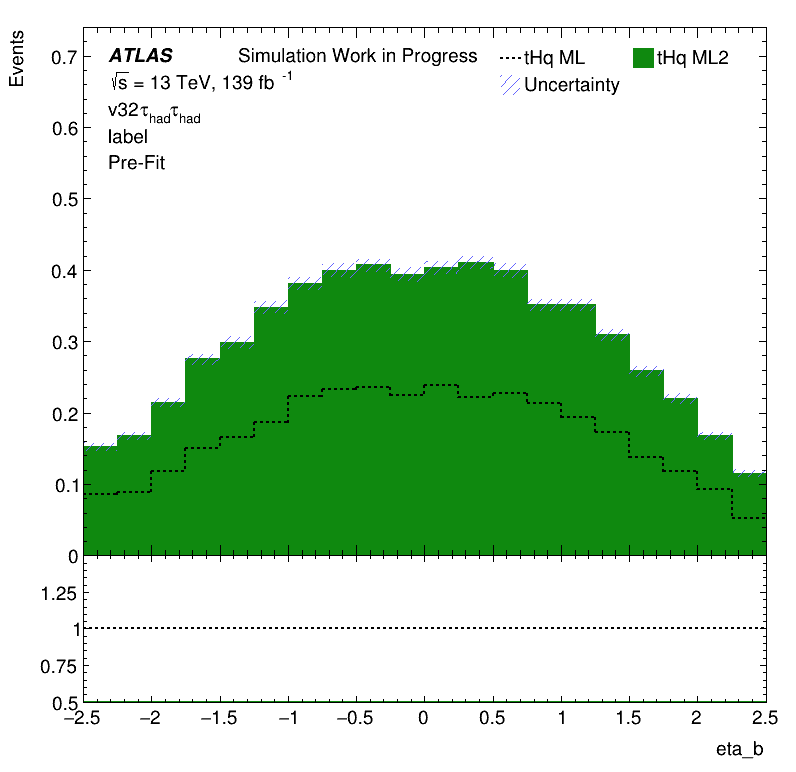
\includegraphics[width=0.8\textwidth]{eta_b}
      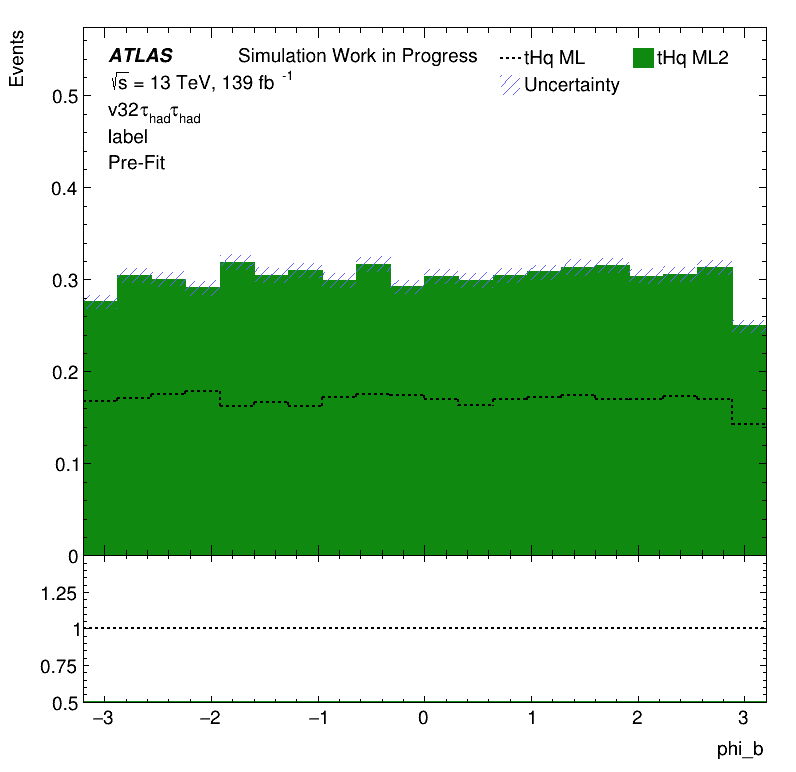
\includegraphics[width=0.8\textwidth]{phi_b}
    \end{column}
    \begin{column}{0.5\textwidth}
      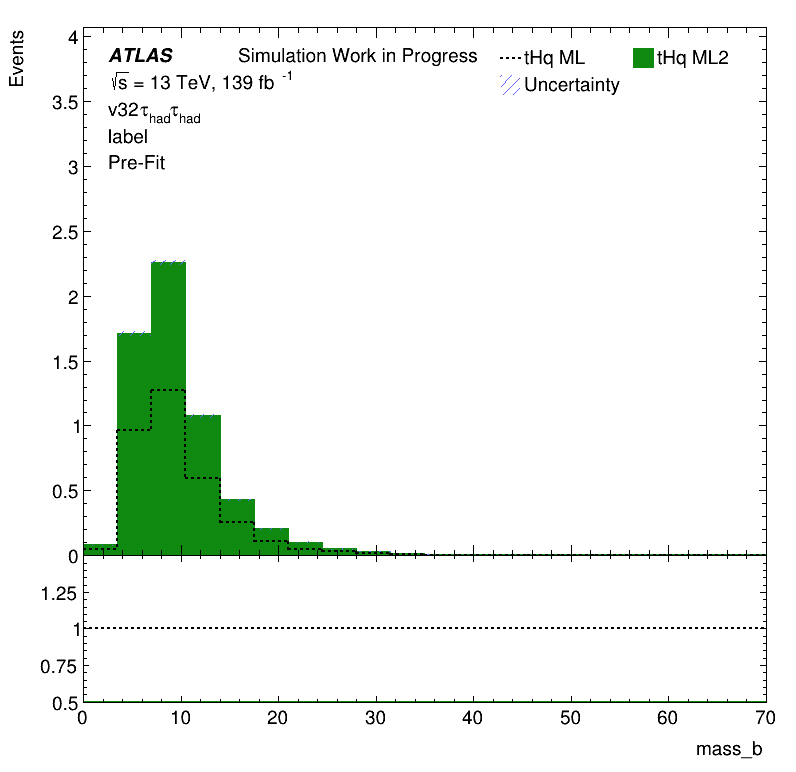
\includegraphics[width=0.8\textwidth]{mass_b}
      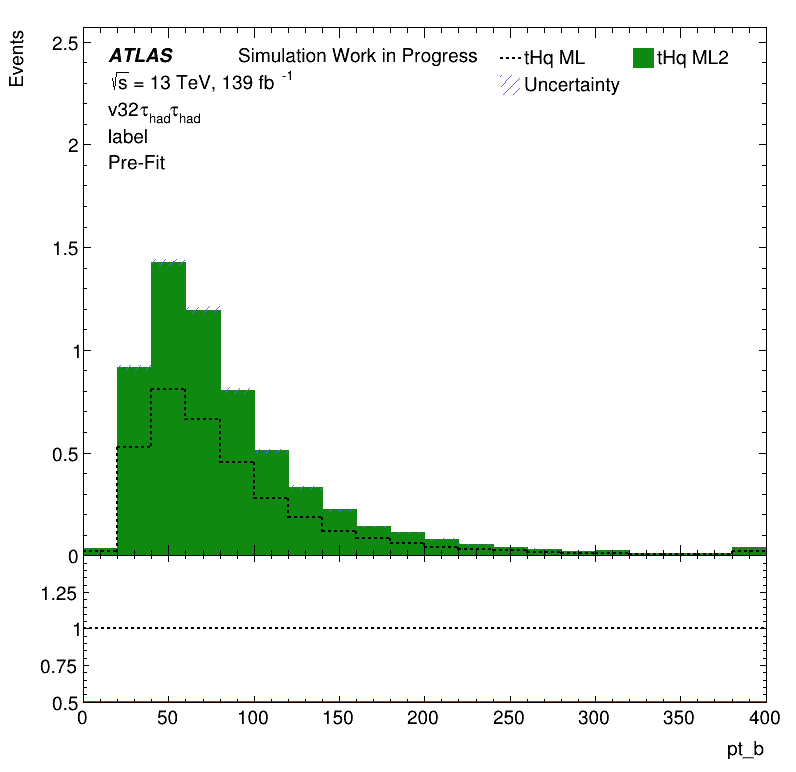
\includegraphics[width=0.8\textwidth]{pt_b}
    \end{column}
  \end{columns}
\end{frame}


\begin{frame}{Monitoring lephad}
\begin{columns}
  \begin{column}{0.5\textwidth}
    \begin{figure}
      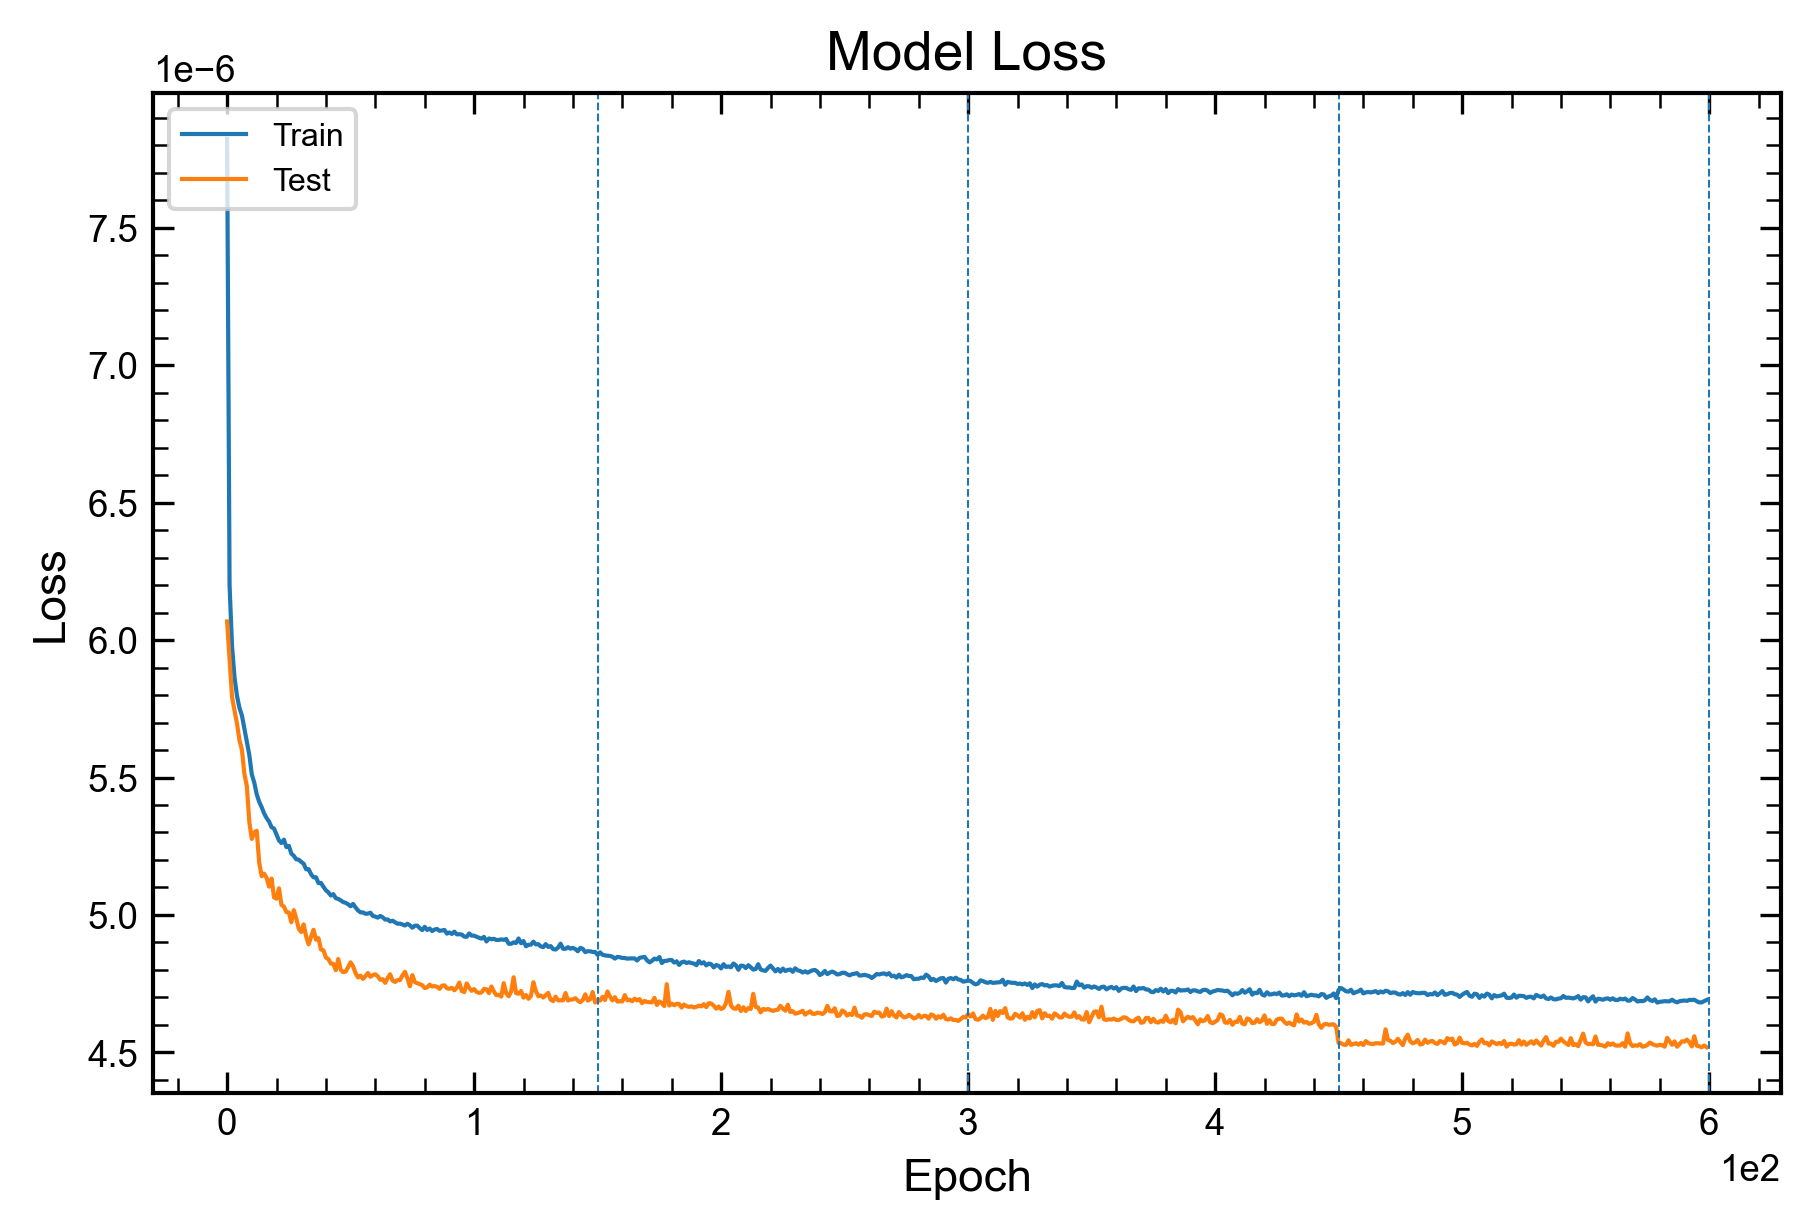
\includegraphics[width=\textwidth]{loss_lephad.png}
    \end{figure}
  \end{column}
  \begin{column}{0.5\textwidth}
    \begin{figure}
      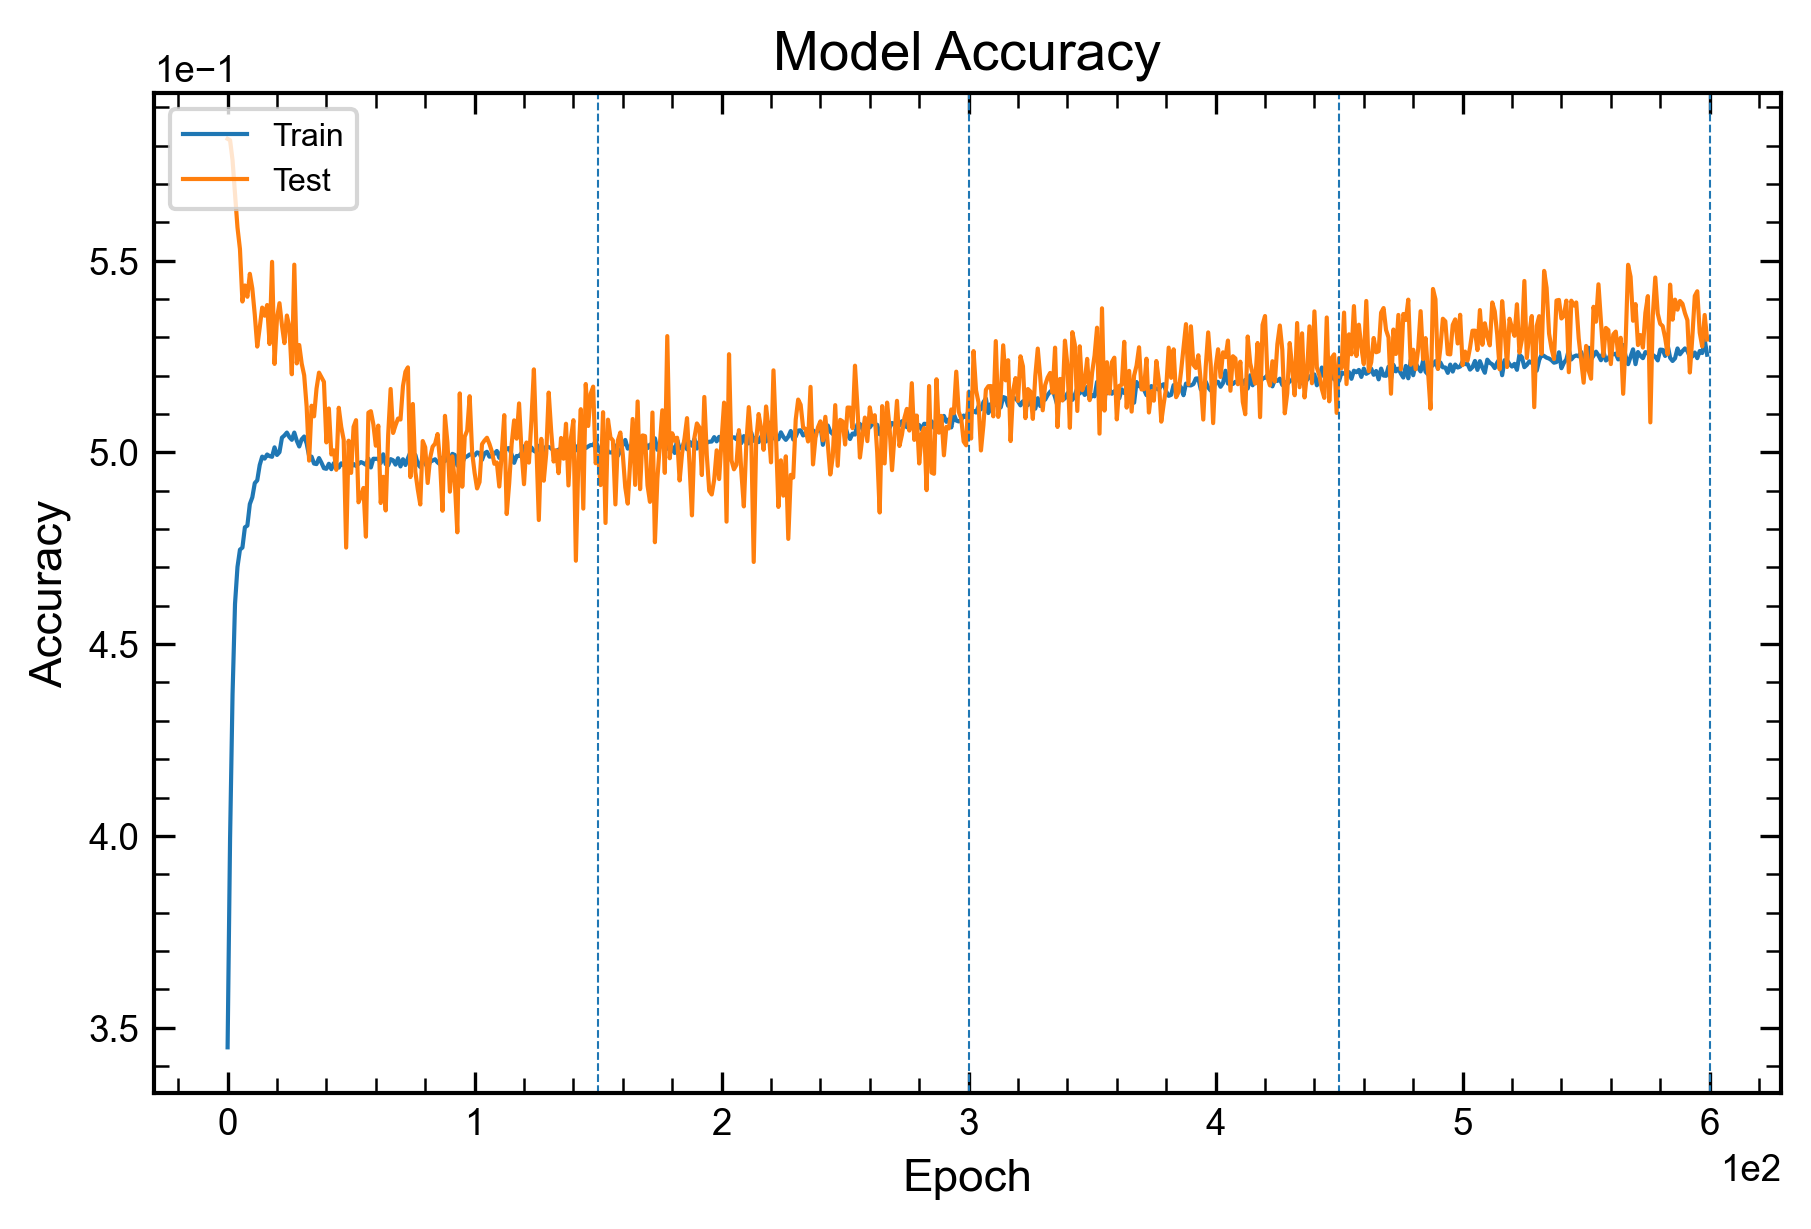
\includegraphics[width=\textwidth]{acc_lephad.png}
    \end{figure}
  \end{column}
\end{columns}
\end{frame}

\begin{frame}{Results lephad}
\begin{columns}
  \begin{column}{0.5\textwidth}
    \begin{figure}
      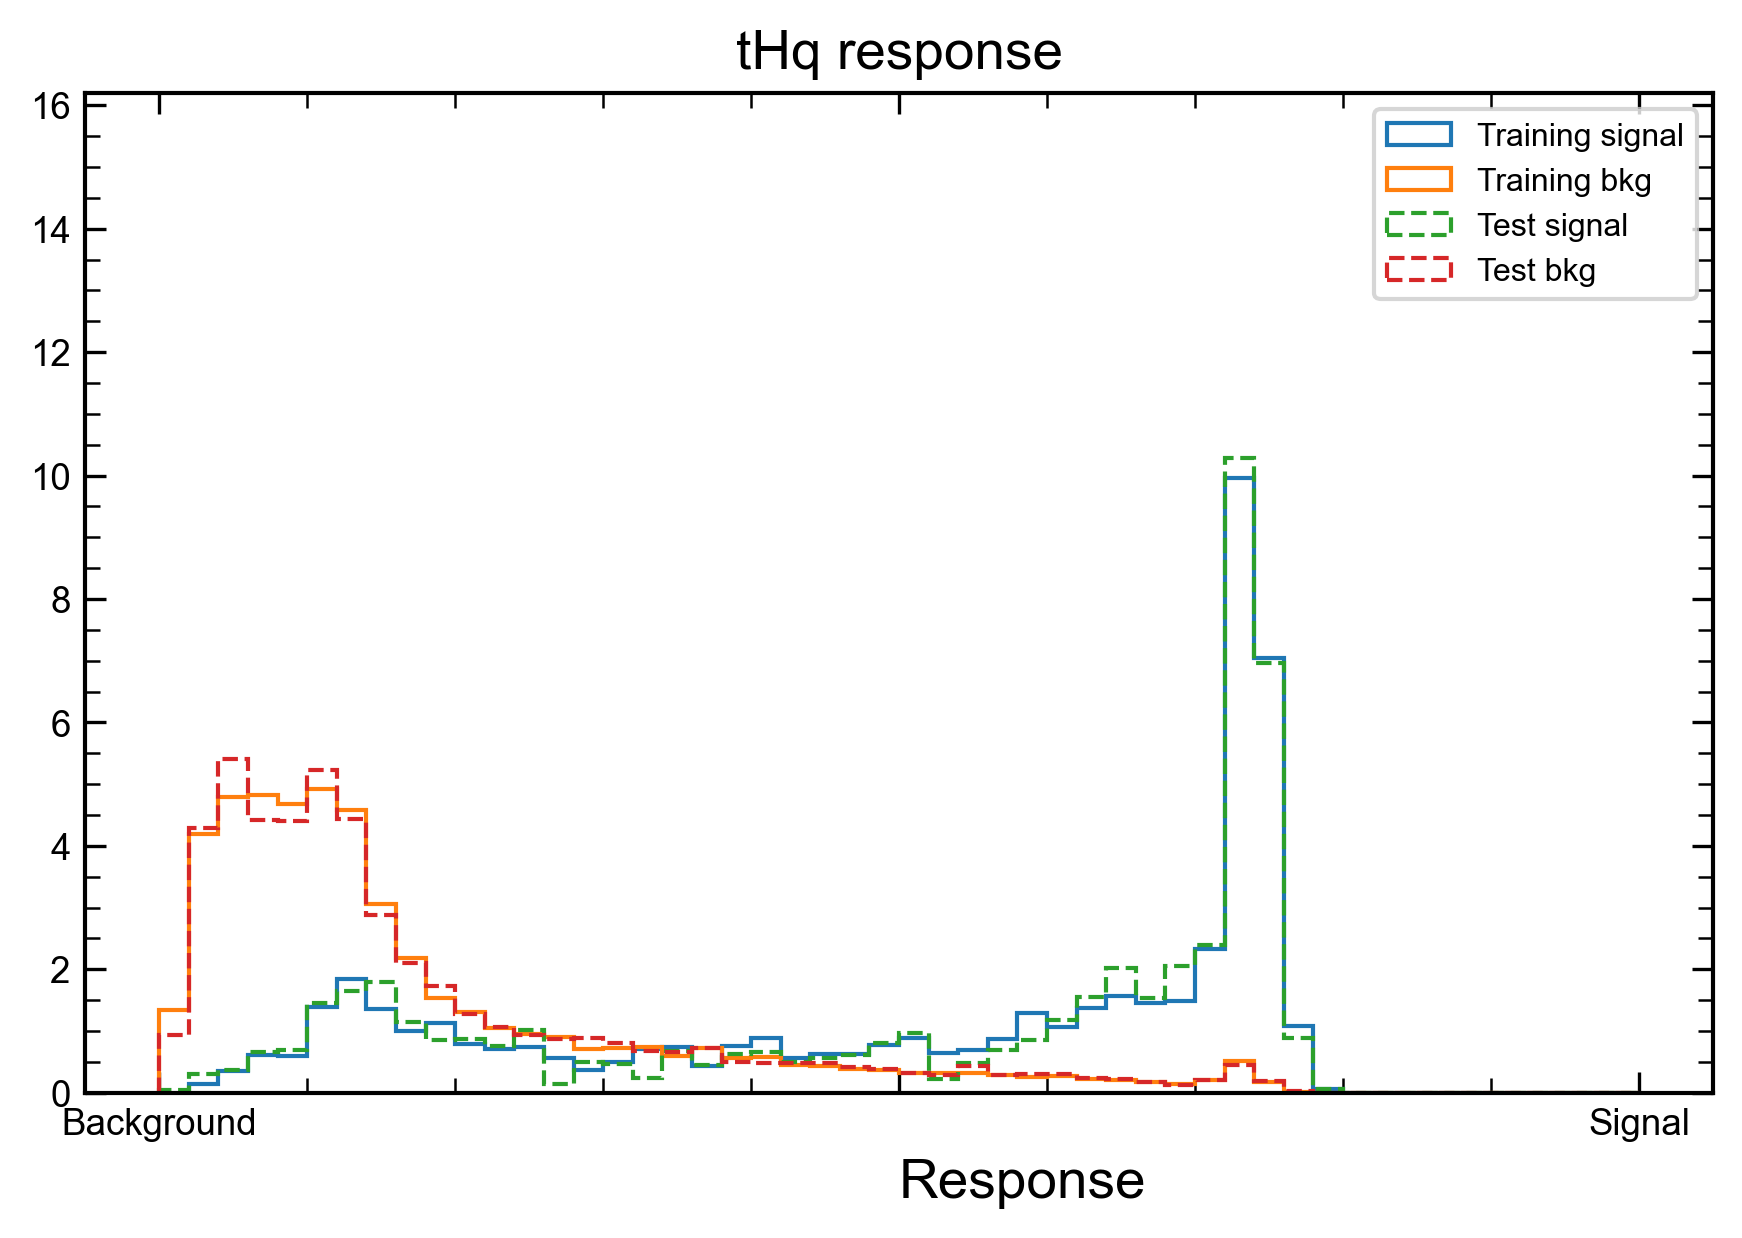
\includegraphics[width=\textwidth]{response_lephad.png}
    \end{figure}
  \end{column}
  \begin{column}{0.5\textwidth}
    \begin{figure}
      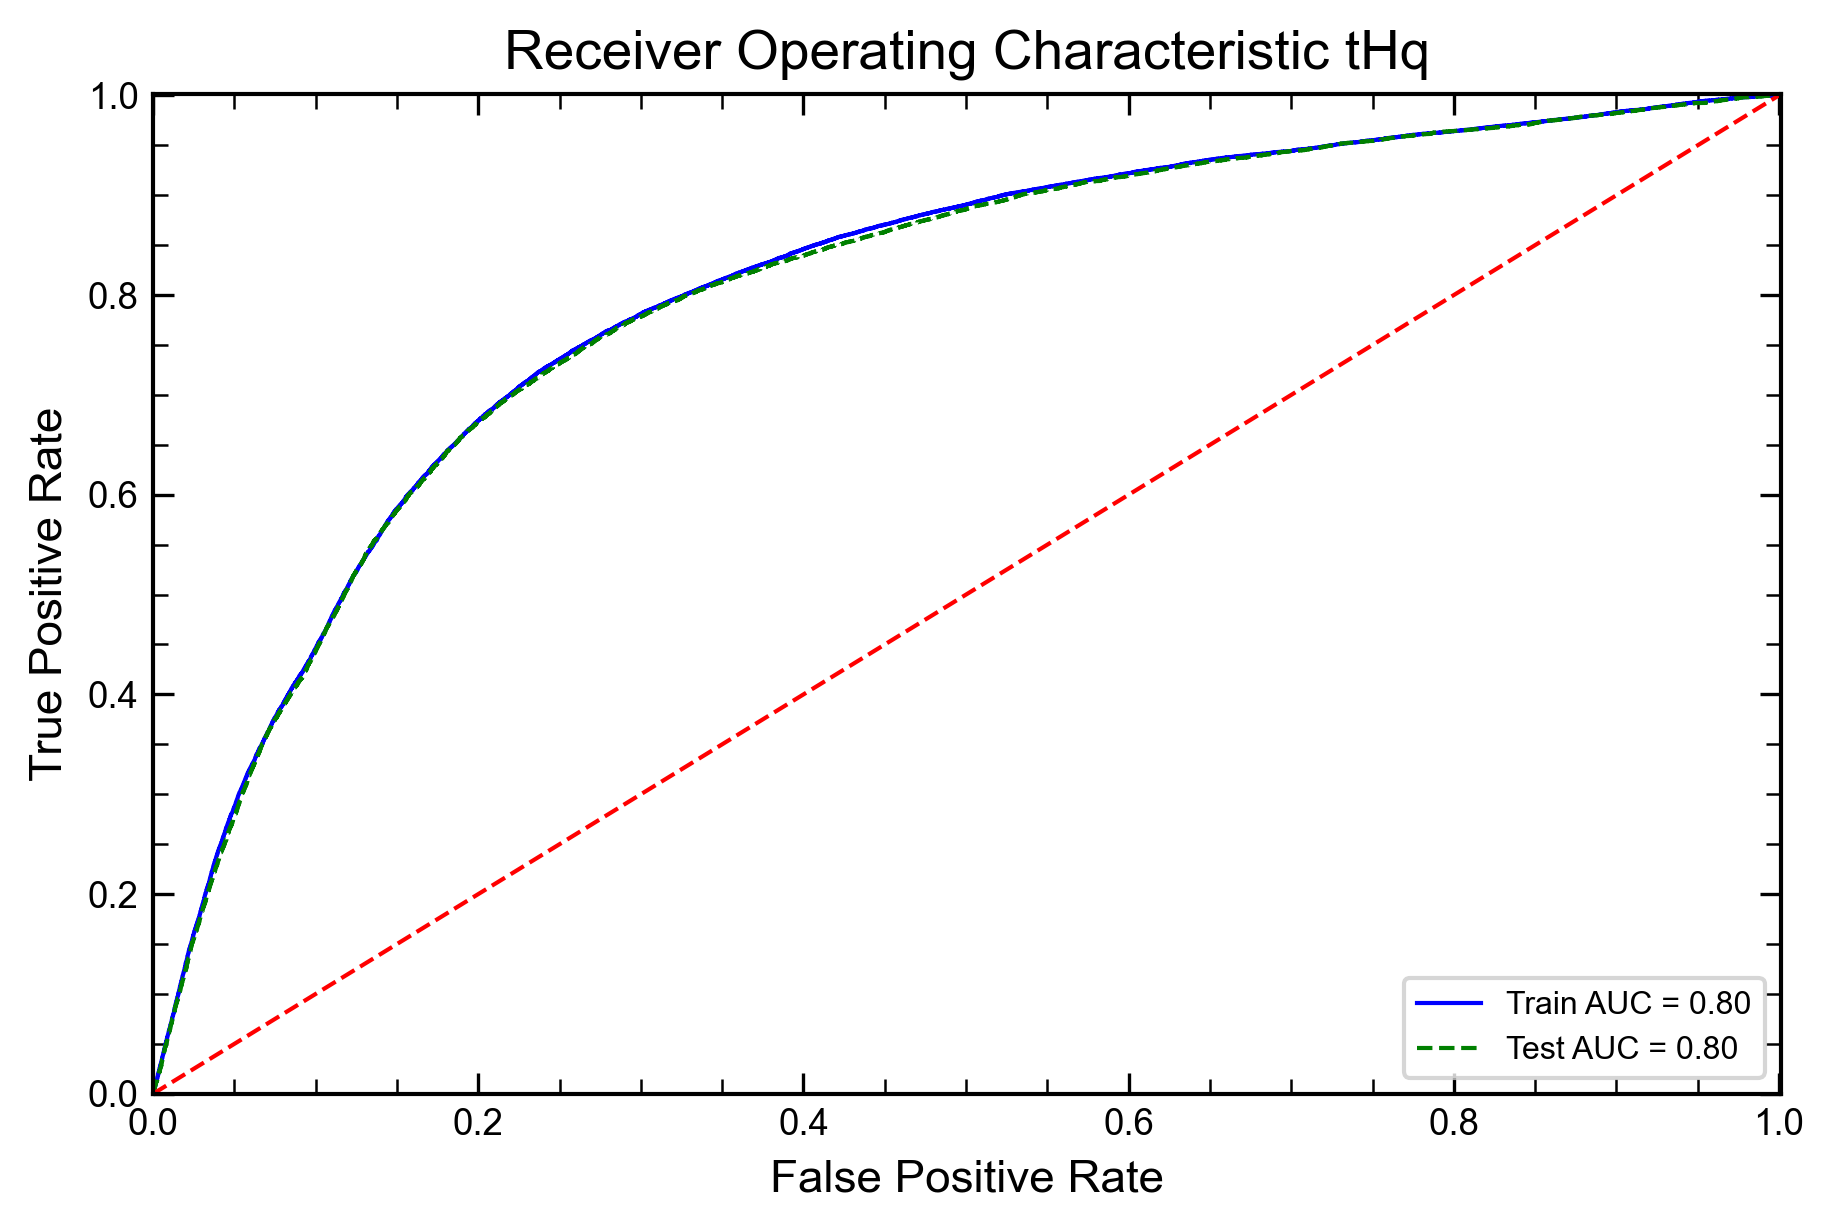
\includegraphics[width=\textwidth]{ROC_lephad.png}
    \end{figure}
  \end{column}
\end{columns}
\end{frame}